\documentclass{article}
\usepackage[utf8]{inputenc}
\usepackage{amsmath}
\usepackage{graphicx}
\usepackage{float}
\usepackage[font=scriptsize,labelfont=bf]{caption}

\title{COMP6245 : Lab 6}
\author{Thanakorn Panyapiang(tp2n19@soton.ac.uk)}
\date{}

\begin{document}
\maketitle

\section{Lab 1 - 5}
I have completed all the five assignments, submitted reports and have taken on board any feedback provided.

\section{K-Means Clustering}
The sample data below is drawn from 3 Gaussian densities where all distributions have approximately the same amount of data.\\
\begin{center}
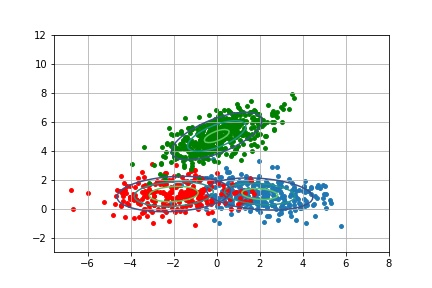
\includegraphics[scale=0.3]{distribution-balance}
\captionof{figure}{Data from a mixture of Gaussian density}
\end{center}

Running 2 versions K-Means clustering(self-implementation and sklearn) on the dataset in Figure 1 gives the result as shown in Figure 2. Based on the prior knowledge about the data, the cluster centroids produced by both versions are consistent with the centers all 3 densities.
\begin{center}
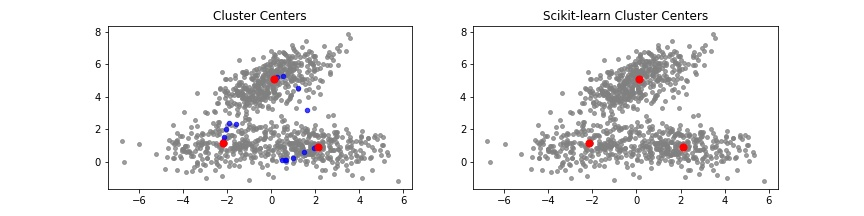
\includegraphics[scale=0.4]{sklean-compare-balance}
\captionof{figure}{}
\end{center}

However, when running both versions of K-Means algorithm on the imbalance dataset displayed in Figure 3, both versions run into the same issue. From the result in Figure 4. , it can be noticed that K-Means locates two centroids on the majority class and one of the minor classes is not considered as a cluster.
\begin{center}
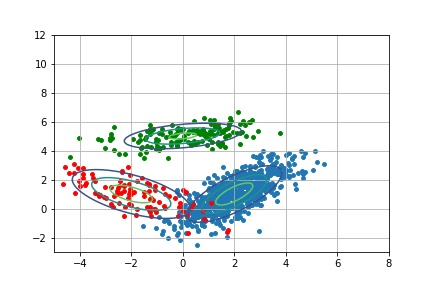
\includegraphics[scale=0.3]{distribution-imbalance}
\captionof{figure}{Imbalance dataset where one density has significantly more data than others}
\end{center}
\begin{center}
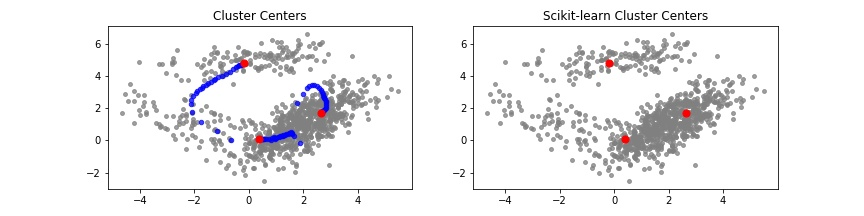
\includegraphics[scale=0.4]{sklean-compare-imbalance}
\captionof{figure}{Results of K-Means clustering on the data in Figure 3}
\end{center}

\section{K-Means Parameters Impact}
This section of the report will analyze the impact of two parameters of K-Means algorithm : \textit{K} and \textit{the initial centroids}.

\subsection{Choice of K}
The result of running K-Means clustering(self-implemented version) on the dataset in Figure 1. with various choices of K is shown in the figure below. What can be observed from the result is that as the value of K increases the size of cluster and the inter-cluster distance become smaller. However, too high value of K could also makes the cluster lack of generalization. For instance, on K = 7, the algorithm divides one density on the top into two groups and two densities below into four clusters.
\begin{center}
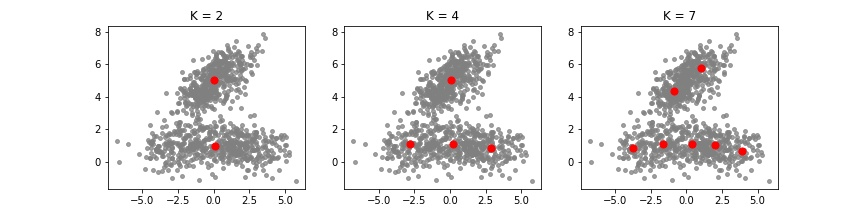
\includegraphics[scale=0.4]{multiple_k}
\captionof{figure}{Clustering results for different values of K}
\end{center}

To choose a proper K, one of the well-known techniques is to use the \textit{Elbow Curve} which is the graph where X-axis represents the value of K and Y-axis represents average distance to centroid as displayed in Figure 6. From the elbow curve, K = 3 is the elbow of the curve which indicates the optimal value of K.\\
\begin{center}
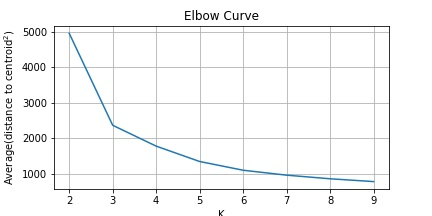
\includegraphics[scale=0.3]{elbow}
\captionof{figure}{}
\end{center}

\subsection{Initial Centroids}

Initial centroids are another factor which has a huge impact on K-Means. The poor selection of centroids could leads to the algorithm returns incorrect results as illustrated in the figure below. In Figure 7a and 7b, there is one initial centroid which is the furthest and the closest to all datapoints respectively.\\

\begin{center}
\begin{tabular}{c c}
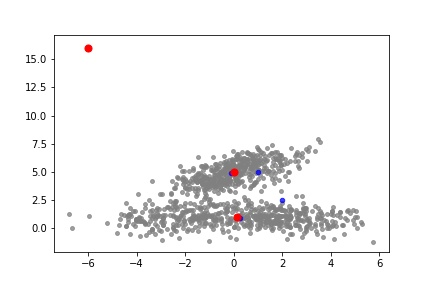
\includegraphics[scale=0.3]{one_furthest_centroid} &
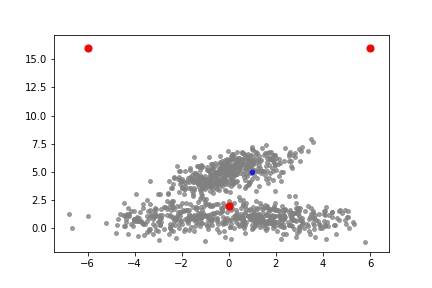
\includegraphics[scale=0.3]{one_nearest_centroid} \\
\scriptsize (a) & \scriptsize (b)
\end{tabular}
\captionof{figure}{}
\end{center}

The cause of this issue is the Expectation-Maximizatioin algorithm, which is the key of K-Means, stucks at the local minimum. In Figure 7a, no data is assigned to the top centroid in the first iteration. Therefore, when K-Means re-average the centroid to minimize the total inter-cluster distance and maximize the likelihood, the top centroid does not move and the algorithm ends up with one empty cluster even though the K is correct. The similar situation also occurs on the Figure 7b where all samples are assigned to the bottom centroid.

One of the popular techniques for choosing initial centroids is to uniformly pick K points in the dataset as an initial centroid. Although this could reduce the chance, this method does not guarantee that the algorithm will not stuck at the suboptimal solution. The more sophisticated approach for this is \textit{k-means++}\cite{kmpp} which is based on the same princleple but using weighted probability distribution instead of uniform sampling.

\section{Testing with the UCI dataset}
In this section, we will verify our K-Means implementation on the Iris dataset from UCI repository. The dataset contains 3 classes where each sample has 4 features and distributes as follow.
\begin{center}
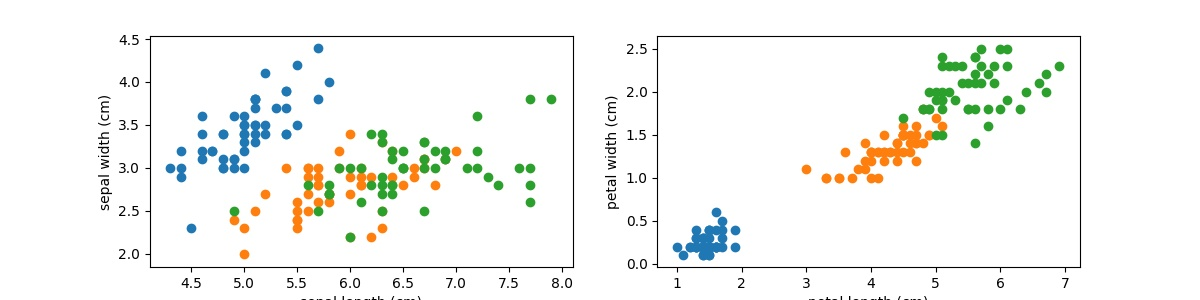
\includegraphics[scale=0.3]{iris_dist}
\captionof{figure}{}
\end{center}
Using K-Means(with K = 3) to cluster the dataset gives the cluster centroids displayed in Figure 9. The result is matched with the dataset description.
\begin{center}
\begin{tabular}{c c}
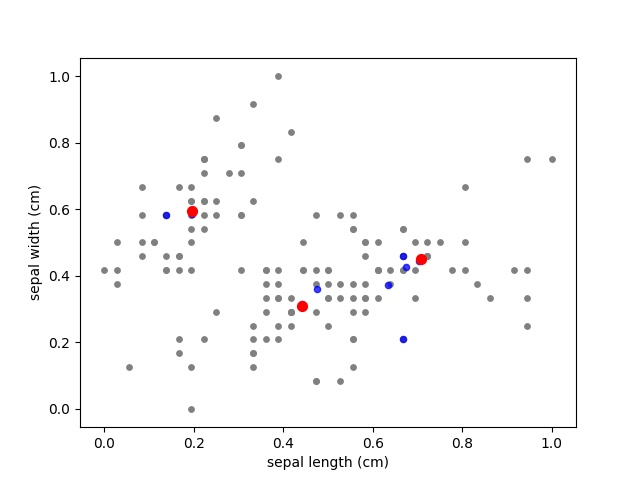
\includegraphics[scale=0.3]{iris_cluster_1} &
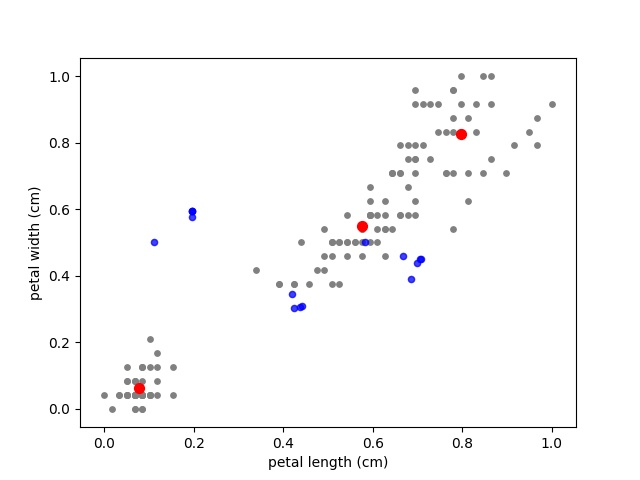
\includegraphics[scale=0.3]{iris_cluster_2} \\
\scriptsize (a) & \scriptsize (b)
\end{tabular}
\captionof{figure}{}
\end{center}

\medskip
 
\begin{thebibliography}{1}
\bibitem{kmpp} 
D. Arthur and S. Vassilvitskii, 
\textit{k-means++: The Advantages of Careful Seeding}.
Proceedings of the eighteenth annual ACM-SIAM symposium on Discrete algorithms. Society for Industrial and Applied Mathematics Philadelphia, 322(10):891921, 2007.

\end{thebibliography}

\end{document}

@article{kmpp,
author = {},
title = {k-means++: The Advantages of Careful Seeding},
journaltitle = {Proceedings of the eighteenth annual ACM-SIAM symposium on Discrete algorithms. Society for Industrial and Applied Mathematics Philadelphia},
year = {2007},
}